\chapter [Deployment and Results]{Deployment and Results}

\section{Test Configurations}
In order to test the proposed architecture, three different configurations have been selected. The first configuration is using just one laser sensor. The second configuration is based on multiple laser sensors, Finally, the third configurations uses multiple lasers along with a camera.

Each configuration consists of a set of processing blocks (as described in section \ref{proc_blocks}) connected, aiming to take data from sensors, lasers and cameras, to produce an output of higher level. In this case, vehicle counting and intersection occupation level are the metrics used for evaluation.

The following table lists all used blocks and assigns an ID for each one. Those IDs are used in the graph description in its own section. Also, bold nodes and connections indicate multiple instance of the same element.

\begin{table}[ht!]
\footnotesize
\centering
\begin{tabular}{|c | c| c|}
\hline
\textbf{Block ID} & \textbf{Name} \\
\hline
A & laser\_publisher \\
\hline
B & laser\_bg\_remover \\
\hline
C & laser\_pol2cart \\
\hline
D & laser\_cart\_merge \\
\hline
E & points2clusters \\
\hline
F & clusters\_leg\_counter \\
\hline
G & leg\_counter\_merge \\
\hline
H & clusters2occ\_level \\
\hline
I & occ\_level\_merge \\
\hline
J & laser\_pol2cart \\
\hline
K & points2occgrid \\
\hline
L & occgrid\_merge \\
\hline
M & occgrid\_leg\_counter \\
\hline
N & occgrid2occ\_level \\
\hline
O & camera\_publisher \\
\hline
P & camera\_bg\_remover \\
\hline
Q & camera\_object\_filter \\
\hline
R & camera\_object2occgrid \\
\hline
\end{tabular}
\caption{Description of processing blocks used in test configurations}
\label{desc_test_config}
\end{table}


\subsection{Case 1: Single Laser}

\begin{figure}[ht!]
\centering
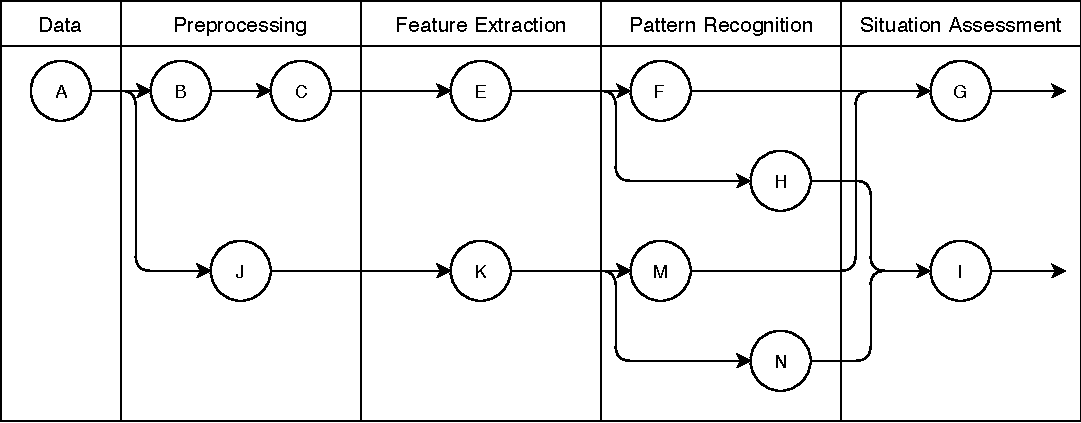
\includegraphics[scale=0.7]{fig/4/test_configuration1.pdf}
\caption{Single laser configuration}
\label{tconf1}
\end{figure}

TODO


\subsection{Case 2: Multiple Lasers}

\begin{figure}[ht!]
\centering
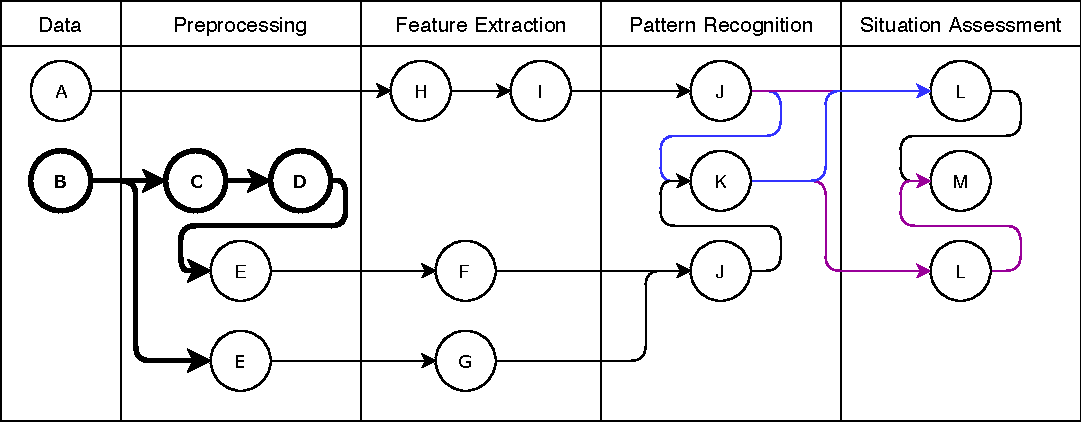
\includegraphics[scale=0.7]{fig/4/test_configuration2.pdf}
\caption{Single laser configuration}
\label{tconf2}
\end{figure}

TODO

\subsection{Case 3: Multiple Lasers and camera}

\begin{figure}[ht!]
\centering
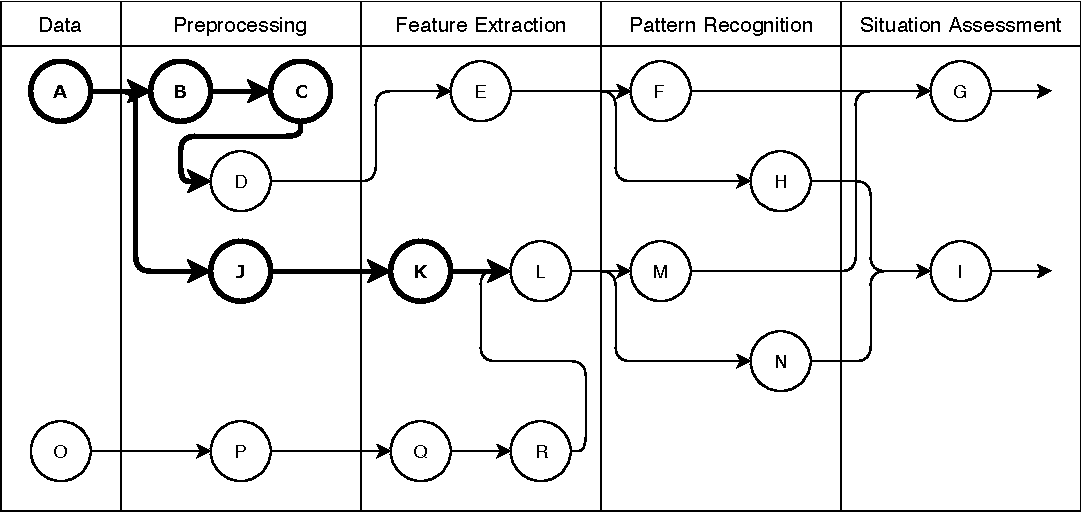
\includegraphics[scale=0.7]{fig/4/test_configuration3.pdf}
\caption{Single laser configuration}
\label{tconf3}
\end{figure}

TODO

\subsection{Results and Comparison}

TODO